\documentclass[aspectratio=169,11pt]{beamer}
\usepackage[T1]{fontenc}
\usepackage{lmodern,amsmath,amssymb,mathtools,bm,booktabs,array,graphicx,tikz}
\usetikzlibrary{arrows.meta,positioning,calc,decorations.pathreplacing,patterns}
\definecolor{ink}{HTML}{17344D}\definecolor{accent}{HTML}{087E8B}\definecolor{pale}{HTML}{EDF5F5}\definecolor{gold}{HTML}{AD6B19}
\providecommand{\dd}{\,\mathrm{d}}\providecommand{\R}{\mathbb{R}}
\providecommand{\E}{\mathbb{E}}\providecommand{\Var}{\operatorname{Var}}
\providecommand{\Cov}{\operatorname{Cov}}\providecommand{\diag}{\operatorname{diag}}
\providecommand{\norm}[1]{\left\lVert#1\right\rVert}
\providecommand{\abs}[1]{\left|#1\right|}
\usefonttheme{professionalfonts}
\setbeamercolor{normal text}{fg=black,bg=white}
\setbeamercolor{frametitle}{fg=ink,bg=white}
\setbeamercolor{title}{fg=ink}\setbeamercolor{structure}{fg=accent}
\setbeamercolor{block title}{fg=ink,bg=pale}\setbeamercolor{block body}{fg=black,bg=pale!40}
\setbeamercolor{alerted text}{fg=accent}
\setbeamerfont{frametitle}{size=\Large,series=\bfseries}
\setbeamerfont{title}{size=\LARGE,series=\bfseries}
\setbeamertemplate{navigation symbols}{}
\setbeamersize{text margin left=.7cm,text margin right=.7cm}
\setbeamertemplate{frametitle}{\vspace{.18cm}\insertframetitle\par\vspace{.1cm}{\color{accent}\hrule height .6pt}\vspace{.12cm}}
\newcommand{\notestarget}{notes.pdf}\newcommand{\noteslabel}{Notes}
\setbeamertemplate{footline}{\hspace{.7cm}\color{ink}\scriptsize Computational Cardiology\quad\href{\notestarget}{\noteslabel}\hfill\insertframenumber\,/\,\inserttotalframenumber\hspace{.7cm}\vspace{.18cm}}
\setbeamercovered{invisible}
\hypersetup{pdfauthor={Zan Ahmad},pdftitle={Implicit pressure equations and ideal-valve complementarity},pdfpagemode=UseNone}
\begin{document}
\begin{frame}[plain]\vfill
{\small\color{accent} Computational Cardiology \quad Lecture 3}\par\medskip
{\raggedright\hyphenpenalty=10000\exhyphenpenalty=10000\LARGE\bfseries\color{ink} Implicit pressure equations and ideal-valve complementarity}\par\bigskip
Zan Ahmad\par\smallskip
{\small Fall 2024}\par\vfill\end{frame}
\renewcommand{\notestarget}{notes.pdf\#note-differentiating-the-constitutive-storage-law}
\begin{frame}[t,fragile,label=slide-the-stored-quantity]{The stored quantity}
\[V=V_d+CP,\qquad \dot V=C\dot P+\dot CP.\]\pause{} Omitting $\dot CP$ removes pressure generation by changing compliance.
\end{frame}
\renewcommand{\notestarget}{notes.pdf\#note-differentiating-the-constitutive-storage-law}
\begin{frame}[t,fragile,label=slide-an-isolated-contracting-compartment]{An isolated contracting compartment}
\[\dot V=0\quad\Longrightarrow\quad CP=\text{constant}.\]\pause{}\[C^{n+1}=C^n/2\quad\Longrightarrow\quad P^{n+1}=2P^n.\]
\end{frame}
\renewcommand{\notestarget}{notes.pdf\#note-the-conductance-laplacian-and-pressure-matrix}
\begin{frame}[t,fragile,label=slide-discretize-stressed-volume]{Discretize stressed volume}
\[C_i^{n+1}P_i^{n+1}-C_i^nP_i^n=h(Bq^{n+1})_i.\]\pause{} Old and new compliance enter at their corresponding time levels.
\end{frame}
\renewcommand{\notestarget}{notes.pdf\#note-the-conductance-laplacian-and-pressure-matrix}
\begin{frame}[t,fragile,label=slide-one-active-connection]{One active connection}
\[q=g(P_i-P_j),\qquad g=1/R.\]\pause{} It contributes $hg\begin{pmatrix}1&-1\\-1&1\end{pmatrix}$ to the two pressure rows.
\end{frame}
\renewcommand{\notestarget}{notes.pdf\#note-the-conductance-laplacian-and-pressure-matrix}
\begin{frame}[t,fragile,label=slide-the-pressure-matrix]{The pressure matrix}
\[(D_C^{n+1}+hBGB^{\mathsf T})P^{n+1}=D_C^nP^n.\]\pause{} Active valves contribute $g=1/R$; closed valves contribute zero.
\end{frame}
\renewcommand{\notestarget}{notes.pdf\#note-the-conductance-laplacian-and-pressure-matrix}
\begin{frame}[t,fragile,label=slide-a-unique-fixed-state-solve]{A unique fixed-state solve}
For $z\ne0$,
\[z^{\mathsf T}Az=\sum_iC_i z_i^2+h\sum_e g_e(z_i-z_j)^2>0.\]\pause{} Positive compliances make $A$ positive definite. Valve consistency is a separate condition.
\end{frame}
\renewcommand{\notestarget}{notes.pdf\#note-ideal-valves-as-a-complementarity-condition}
\begin{frame}[t,fragile,label=slide-the-ideal-valve-law]{The ideal-valve law}
\[q=\frac{\max(d,0)}R,\qquad d=P_{\rm up}-P_{\rm down}.\]\pause{}\[q\ge0,\quad Rq-d\ge0,\quad q(Rq-d)=0.\]
\end{frame}
\renewcommand{\notestarget}{notes.pdf\#note-ideal-valves-as-a-complementarity-condition}
\begin{frame}[t,fragile,label=slide-active-set-iteration]{Active-set iteration}
Choose valve labels, solve the coupled pressure system, then evaluate new pressure differences.\pause{} An inconsistent label changes the matrix and requires another solve.
\end{frame}
\renewcommand{\notestarget}{notes.pdf\#note-a-two-compartment-active-set-calculation}
\begin{frame}[label=slide-a-rejected-closed-candidate-panel-1]{A guessed valve state must be checked}
\centering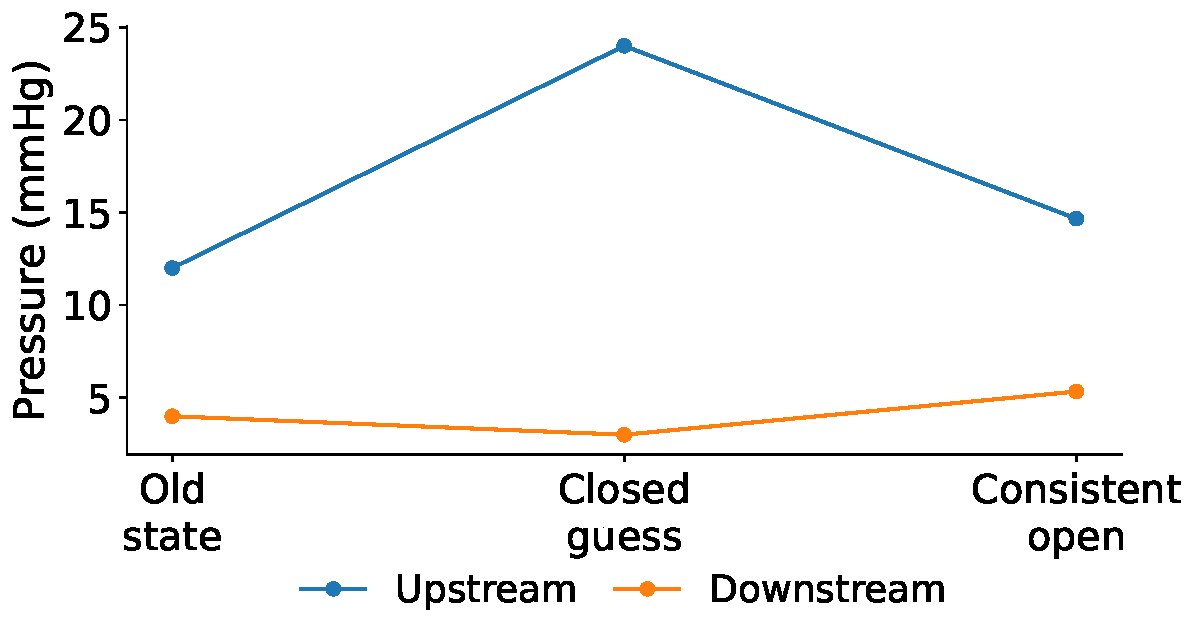
\includegraphics[width=.98\linewidth,height=.69\textheight,keepaspectratio]{presentation-figures/valve-trace-panel-1.pdf}\end{frame}
\renewcommand{\notestarget}{notes.pdf\#note-a-two-compartment-active-set-calculation}
\begin{frame}[label=slide-a-rejected-closed-candidate-panel-2]{Conservation alone cannot choose the valve}
\centering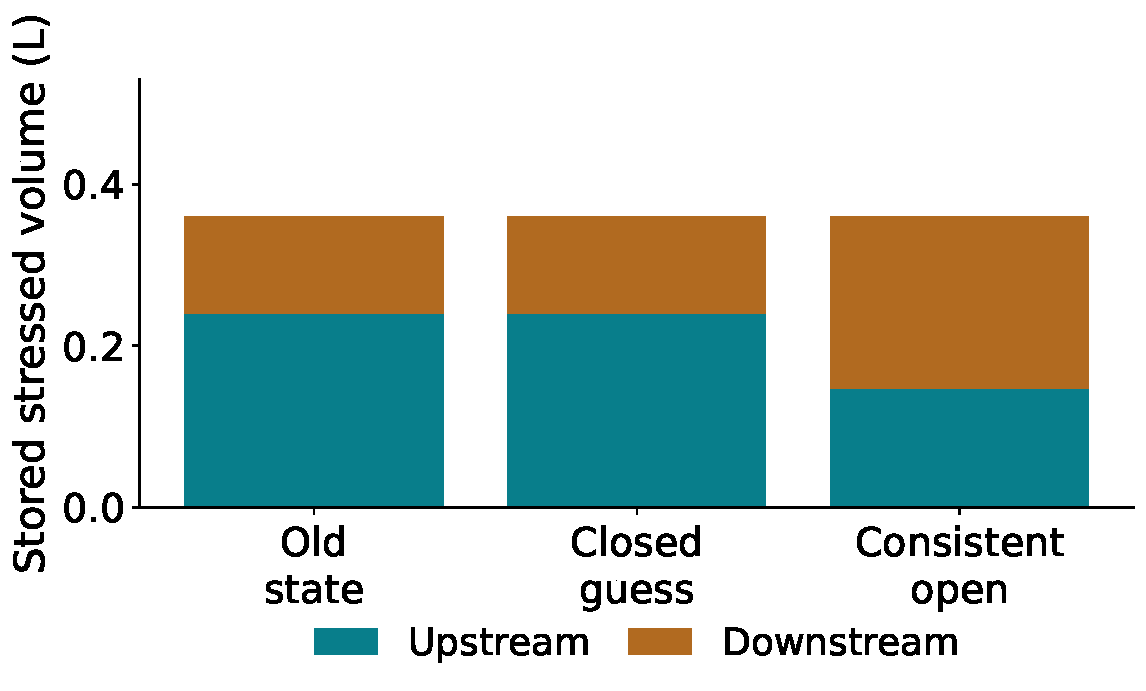
\includegraphics[width=.98\linewidth,height=.69\textheight,keepaspectratio]{presentation-figures/valve-trace-panel-2.pdf}\end{frame}
\renewcommand{\notestarget}{notes.pdf\#note-a-two-compartment-active-set-calculation}
\begin{frame}[t,fragile,label=slide-a-rejected-closed-candidate]{A rejected closed candidate}
Old stressed volumes are $(.24,.12)$ L; new compliances are $(.01,.04)$ L/mmHg.\pause{}\[P_{\rm closed}=(24,3)\ \mathrm{mmHg}.\] Total volume is correct, but $24-3>0$ contradicts closure.
\end{frame}
\renewcommand{\notestarget}{notes.pdf\#note-a-two-compartment-active-set-calculation}
\begin{frame}[t,fragile,label=slide-the-accepted-open-candidate]{The accepted open candidate}
\[\begin{pmatrix}.02&-.01\\-.01&.05\end{pmatrix}P=\begin{pmatrix}.24\\.12\end{pmatrix}.\]\pause{}\[P=(44/3,16/3),\qquad q=14/3\ \mathrm{L/min}.\]
\end{frame}
\renewcommand{\notestarget}{notes.pdf\#note-a-two-compartment-active-set-calculation}
\begin{frame}[t,fragile,label=slide-one-transfer-two-balance-equations]{One transfer, two balance equations}
\[h q=\frac7{75}\ \mathrm L,\qquad V^{n+1}=\left(\frac{11}{75},\frac{16}{75}\right)\mathrm L.\]\pause{} The loss from one compartment equals the gain by the other.
\end{frame}
\renewcommand{\notestarget}{notes.pdf\#note-exact-relaxation-and-backward-euler-error}
\begin{frame}[t,fragile,label=slide-constant-compliance-relaxation]{Constant-compliance relaxation}
For a forward pressure difference $d(0)\ge0$,
\[d=P_1-P_2,\qquad \dot d=-\lambda d,\qquad \lambda=\frac{1/C_1+1/C_2}{R}.\]\pause{}\[d(t)=d(0)e^{-\lambda t}.\]
\end{frame}
\renewcommand{\notestarget}{notes.pdf\#note-exact-relaxation-and-backward-euler-error}
\begin{frame}[t,fragile,label=slide-the-limiting-pressure]{The limiting pressure}
\[P_\infty=\frac{C_1P_1(0)+C_2P_2(0)}{C_1+C_2}.\]\pause{} With $C=(.01,.04)$ and $P(0)=(20,5)$, $P_\infty=8$ mmHg.
\end{frame}
\renewcommand{\notestarget}{notes.pdf\#note-exact-relaxation-and-backward-euler-error}
\begin{frame}[label=slide-backward-euler-and-the-exact-factor-figure]{An implicit conservative update still has time error}
\centering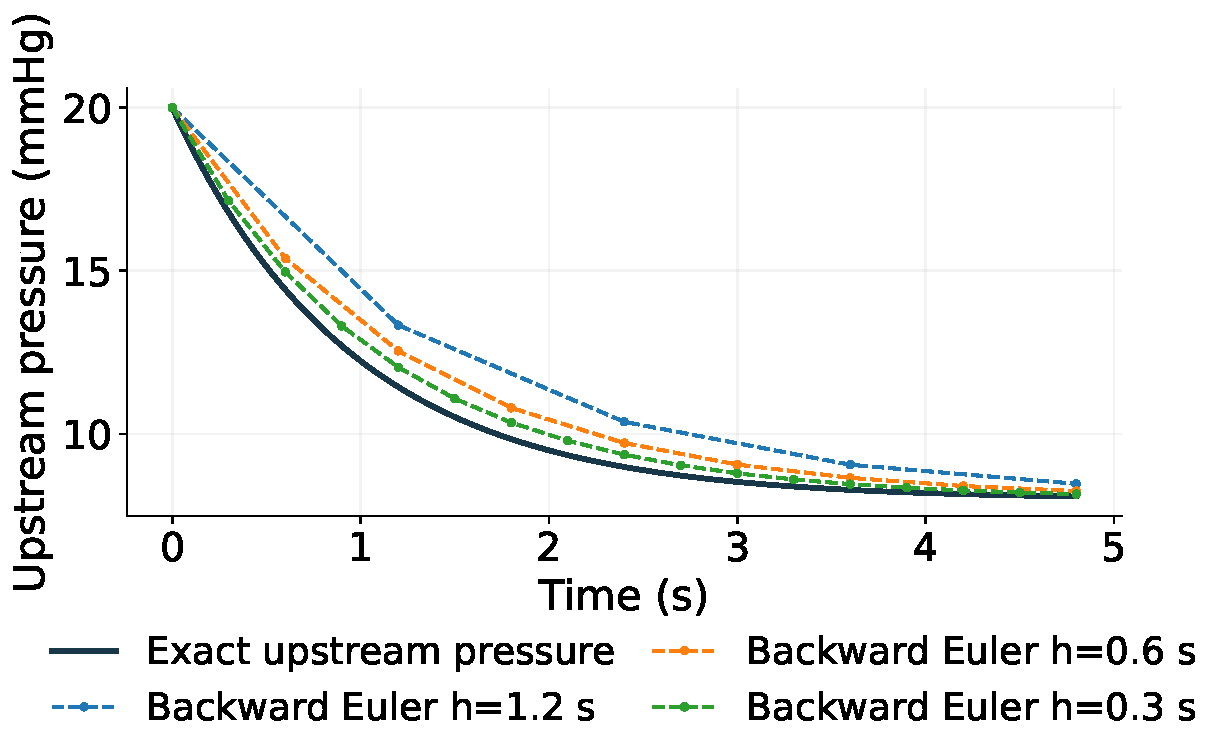
\includegraphics[width=.98\linewidth,height=.69\textheight,keepaspectratio]{presentation-figures/implicit-refinement-panel-1.pdf}\end{frame}
\renewcommand{\notestarget}{notes.pdf\#note-exact-relaxation-and-backward-euler-error}
\begin{frame}[t,fragile,label=slide-backward-euler-and-the-exact-factor]{Backward Euler and the exact factor}
\[d_{n+1}=\frac{d_n}{1+h\lambda},\qquad d(t+h)=e^{-h\lambda}d(t).\]\pause{} Stability does not make the two factors equal.
\end{frame}
\renewcommand{\notestarget}{notes.pdf\#note-extension-to-the-six-compartment-circuit}
\begin{frame}[t,fragile,label=slide-conservation-and-admissibility]{Conservation and admissibility}
A step is accepted only when the storage equations and all valve inequalities hold together.\pause{} Constant-compliance relaxation supplies an exact reference; switching and changing compliance require their own error analysis.
\end{frame}
\end{document}
